\chapter{Implementation}
\thispagestyle{empty}
The suspicious text detection system implementation consist of different modules. In this chapter we will see the implementation details of this modules. Finally we will see sample input and output of our system.

\section{System Requirements}
Our system takes Bengali text as input and classifies it as suspicious or non-suspicious. To implement this system some hardware and software tools are needed. Required hardware and software tools are listed below.
\subsection{Hardware Requirements}
From input to output the system propagate the following hardware :
\begin{itemize}
    \item Nvidia GeForce GTX 1070 GPU
    \item Minimum GPU RAM 8GB
    \item Physical memory 32GB
    \item Intel core i7-7700K CPU
    \item Solid State Drive (SSD) 256GB
    \item Minimum 2h backup UPS
    \item GPU cooler
    \item Monitors
\end{itemize}
\clearpage
\subsection{Software Requirements}
We implement our system in a specific software environment. Required software lists are,

\begin{itemize}
    \item Operating System : ubuntu 16.04, windows 10
    \item Python 3.0
    \item tensorflow-gpu==1.3.0
    \item djangorestframework==3.7.7
    \item numpy==1.12.1
    \item Django==1.11
    \item Pygments==2.2.0
    \item Markdown==2.6.10
    \item coreapi==2.3.3
    \item psycopg2==2.7.3.2
    \item dj-database-url==0.4.2
    \item gunicorn==19.7.1
    \item whitenoise==3.3.1
    \item django-filter==1.1.0
    \item drf-extensions==0.3.0
    \item spyder 3.6
    \item jupyter notebook
\end{itemize}
\par
\vspace{0.5cm}
\noindent
All of this softwares are not required at a time. To implement different part of our system this softwares were used. To test our system one just need an IDE where the system could be run.

\clearpage
\section{Implementation Details}
We implement the system at different steps from training to testing. These steps are,
\subsection{Training Corpus}
Training corpus is key to suspicious text detection system. No pre-build corpus is available for suspicious Bangla text. We build the corpus and it takes six months to collect data form different online and offline sources. Our training corpus is divided into two folder one is for suspicious and another is for non suspicious text. \textbf{Fig.} \ref{fig:CAP} shows categorical folder of our system.
\begin{figure}[h!]
    \centering
    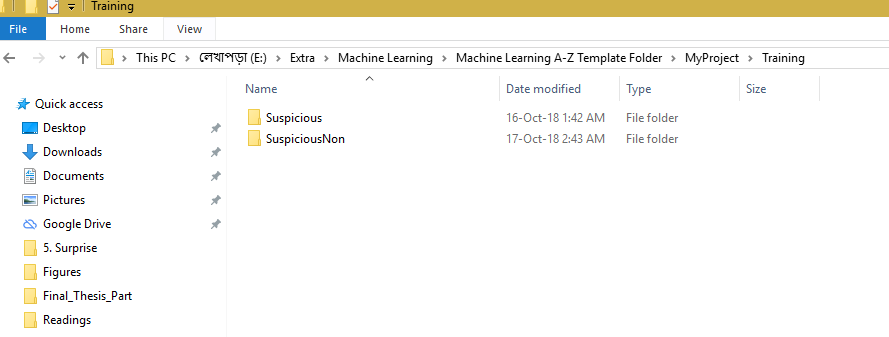
\includegraphics[scale=0.6]{Figures/categorical_fld.PNG}
    \caption{Categorical Folder}
    \label{fig:CAP}
\end{figure}
\par\noindent
\vspace{0.5cm}
\textbf{Fig.}\ref{fig:SMT} shows sample training texts of our system.
\begin{figure}[h!]
    \centering
    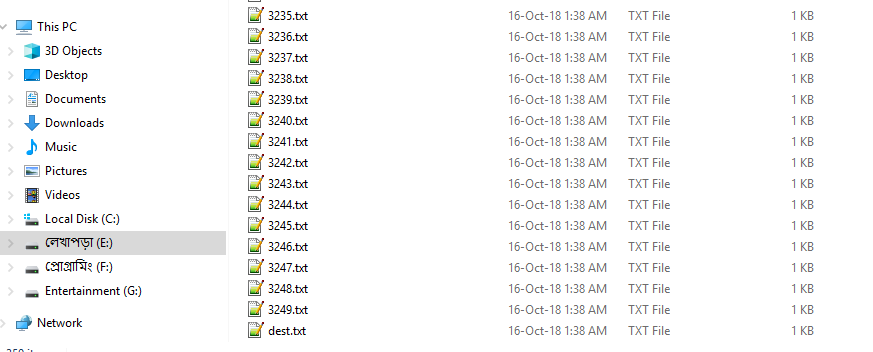
\includegraphics[scale=0.6]{Figures/sample_train.PNG}
    \caption{Sample Training Texts}
    \label{fig:SMT}
\end{figure}

\subsection{Stopword List}
\textbf{Fig.} \ref{fig:stpw} shows a list of some stopword.
In our system the words which has no contribution to classify text is referred as stopwords. From our training text such stopwords were removed. 635 stopwords were collected, from which a list of stopword was built. Removal of this unnecessary words help to increase efficiency of our system.


\begin{figure}[h!]
    \centering
    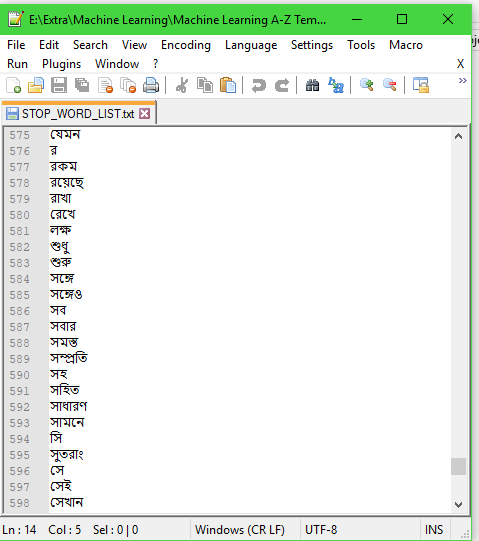
\includegraphics[scale=0.55]{Figures/stp_wrd.PNG}
    \caption{Sample Stopword}
    \label{fig:stpw}
\end{figure}
\par\noindent

\textbf{Fig.} \ref{fig:lstpw} shows the list of stopwords after loading them into our system environment.
\begin{figure}[h!]
    \centering
    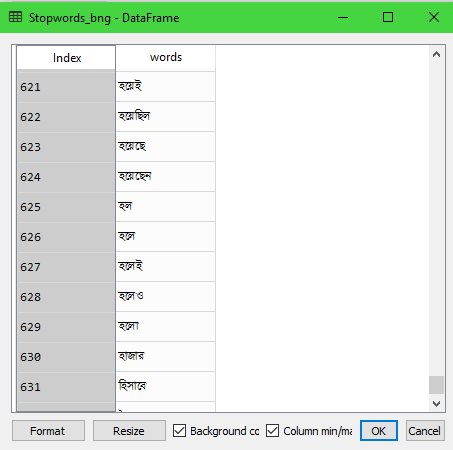
\includegraphics[scale=0.6]{Figures/lstp_wrd.PNG}
    \caption{Stopword in System Environment}
    \label{fig:lstpw}
\end{figure}
\subsection{Processed Corpus}
Processed corpus is the list of all processed text from which we are ready to extract feature. A processed corpus can be created by following steps,
\begin{itemize}
    \item Tokenization of a text.
    \item Punctuation and stopword removal.
    \item Append back remaining words in the text.
\end{itemize}
\textbf{Fig.} \ref{fig:tkn} shows tokenization of a text.
\begin{figure}[h!]
    \centering
    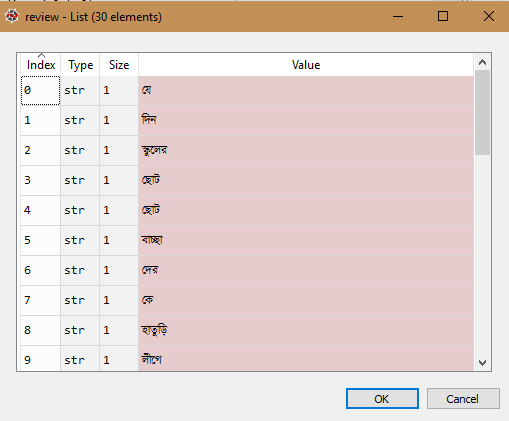
\includegraphics[scale=0.6]{Figures/tokenize.PNG}
    \caption{Tokenized Text}
    \label{fig:tkn}
\end{figure}
\par\noindent
\textbf{Fig.} \ref{fig:crps} shows text corpus in our system environment.
\begin{figure}[h!]
    \centering
    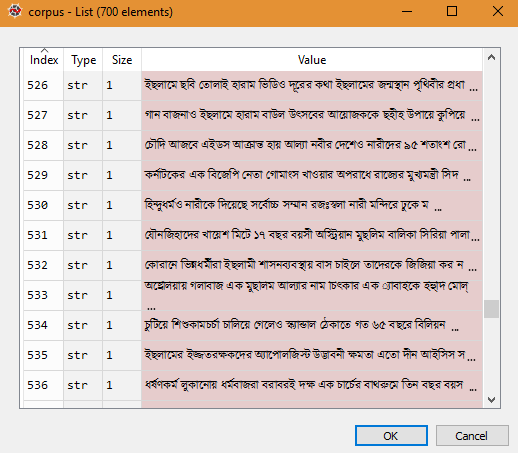
\includegraphics[scale=0.6]{Figures/corpus.PNG}
    \caption{Corpus in System Environment}
    \label{fig:crps}
\end{figure}

\subsection{Corpus Feature}
\textbf{Fig.} \ref{fig:feature} shows a part of our training set feature space.
After processing the texts our next step is to extract feature from the processed text corpus. Feature extraction is an important step because our classifier will learn from the features we extract from texts. More feature will help our classifier model to classify texts more accurately.

\par\noindent
\begin{figure}[h!]
    \centering
    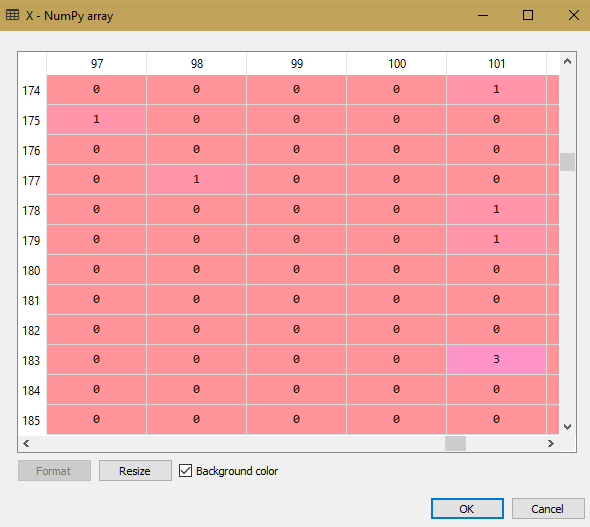
\includegraphics[scale=0.9]{Figures/feature.PNG}
    \caption{Feature Space of Training Set}
    \label{fig:feature}
\end{figure}
\par\noindent
Our feature space is a two dimensional array where rows represents each text of the corpus and columns represents number of unique words available in the corpus. Each cell of the array represents the number of time a specific word occurs in a specific text. 
%\clearpage
\subsection{Labeling of Text}
\textbf{Fig.} \ref{fig:lbt} shows the labeling of texts.
In our system each of the text is labeled with either $0$ or $1$. If the texts are not labeled then the system will not be able to process it. Here $0$ represents suspicious text and $1$ represents non suspicious text. 
\begin{figure}[h!]
    \centering
    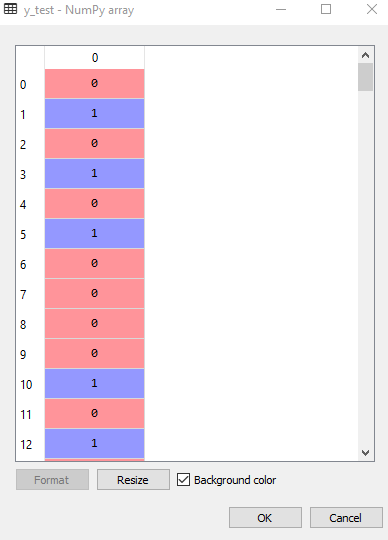
\includegraphics[scale=0.55]{Figures/label_of_text.PNG}
    \caption{Labeling of Texts}
    \label{fig:lbt}
\end{figure}
%\clearpage
\subsection{Prediction of Classifier}
\textbf{Fig.} \ref{fig:prd} shows prediction for a test set.
Our classifier predicts from its learning ability. Each cell of the prediction array represent a prediction for a text. If prediction is $0$ then the text is suspicious otherwise the text is non suspicious.
\begin{figure}[h!]
    \centering
    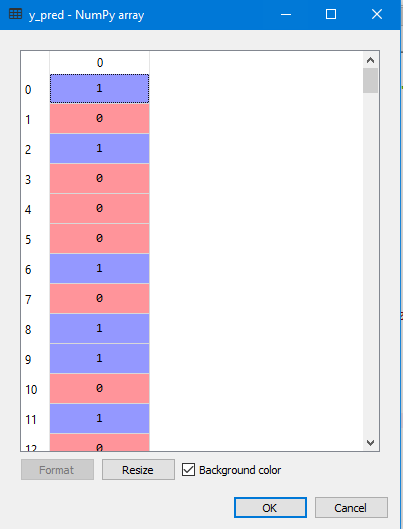
\includegraphics[scale=0.55]{Figures/prediction.PNG}
    \caption{Prediction Array}
    \label{fig:prd}
\end{figure}

\section{Sample Input and Output}
\textbf{Fig.} \ref{fig:smi} shows the inputs of the user in our sample input folder. This is the most important part of our system. We have to check how well our system predict for a sample suspicious and non suspicious text. We will take user inputs in a sample input folder as .txt file. Then this inputs is processed and generate corresponding prediction by our model.\par\vspace{0.5cm}
\begin{figure}[h!]
    \centering
    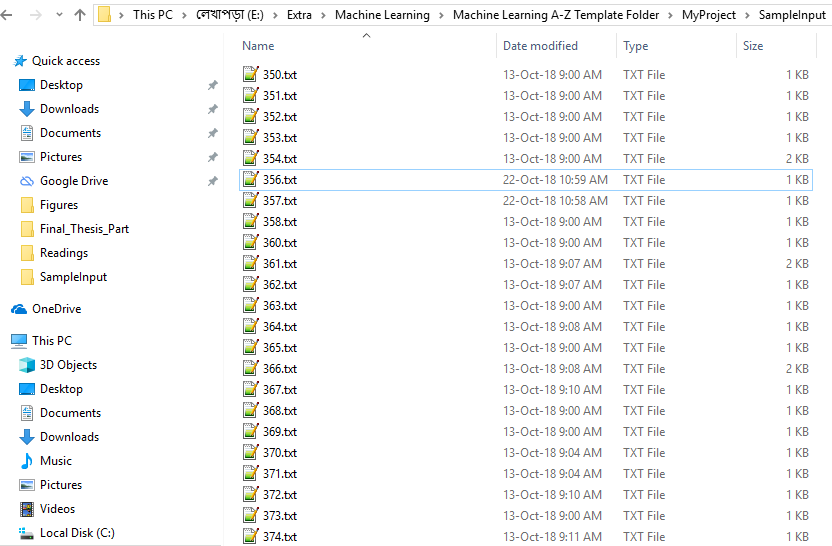
\includegraphics[scale=0.65]{Figures/sample_inp.PNG}
    \caption{Input Folder}
    \label{fig:smi}
\end{figure}
\par\noindent
\vspace{0.3cm}
\textbf{Fig.} \ref{fig:ui} shows a random input of the user.
\begin{figure}[h!]
    \centering
    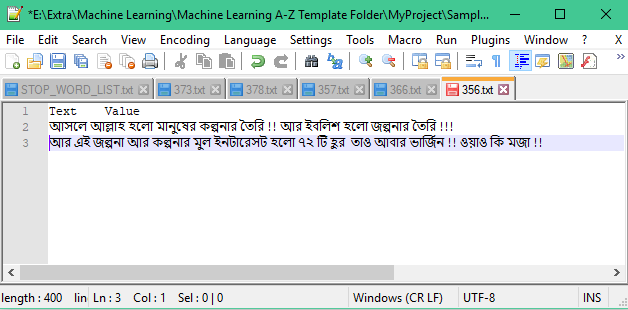
\includegraphics[scale=0.7]{Figures/input_s.PNG}
    \caption{Random Sample Input}
    \label{fig:ui}
\end{figure}
\par\noindent
\textbf{Fig.} \ref{fig:out} shows the prediction of our model. Sample text is user input text and our model predict it as a suspicious or a non suspicious text.
\par
\vspace{1cm}
\begin{figure}[h!]
    \centering
    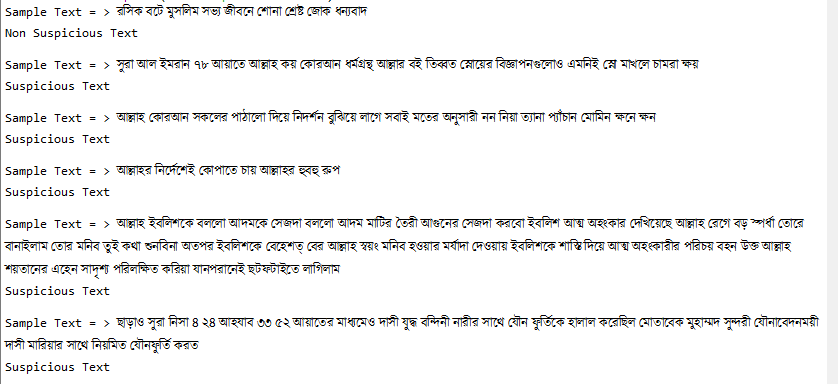
\includegraphics[width=15cm, height=14cm]{Figures/output.PNG}
    \caption{Output in System Environment}
    \label{fig:out}
\end{figure}